% !TEX root =  paper.tex
\section{Background}\label{sec:background}

In this section, we present basic concepts
about E2E test automation that are needed 
to understand the remainder of the paper.
We provide background information on 
DOM-based and visual web testing approaches.
To present these approaches and concepts
we use the example provided in~\autoref{fig:ab-back}: 
a simplified version of the AddressBook web application, 
one of the experimental objects used in our study. 
We consider a scenario in which a user 
inserts a \texttt{username} and \texttt{password} 
in the AddressBook login form 
(\autoref{fig:ab-back-a}), 
and if these credentials are correct, 
the \texttt{username} (\texttt{`admin'}) is displayed on the top right corner of the homepage 
(\autoref{fig:ab-back-b}).

\noindent
\textbf{Approaches to E2E Web Test Automation.}
In recent years, two major approaches to E2E web testing have emerged, each of them associated with a diverse way of interacting with the AUT. 

\textit{DOM-based} tools access and inspect properties of the Document Object Model (DOM), the hierarchical structure underlying a web page. 
%To this category belong capture-replay (C\&R) and programmable tools. \textit{Capture-replay} tools are based on the recording of sequences of inputs and actions performed by the tester on the web application GUI. The recording process creates a test script (see~\autoref{t:seleniumtest}) that can be replayed in a unattended mode. 
%With \textit{programmable} tools, on the other hand, test cases themselves become software artefacts that developers write resorting to specific testing frameworks (see~\autoref{lst:login-no-abs-back}). 
Specific testing framework APIs support the creation of test scripts that automate the interaction with a web page and its elements, and the sequences of inputs and actions performed by the tester on the web application. A test script can, for instance, automatically fill-in and submit forms or click on hyperlinks (see \autoref{fig:ab-back-c}). There are many test automation tools for web applications available, e.g., Selenium~\cite{selenium}, Sahi~\cite{sahi}, and Ringer~\cite{ringer}. %A representative of the programmable category is Selenium WebDriver~\cite{selenium}, which is considered the flagship open-source test automation tool for web applications.

An emerging and relatively new approach is \textit{visual} web testing, in which the AUT is tested through its GUI. Indeed, the emergence of new complex visual components in web pages has required new ways of interfacing with the web applications. Visual tools such as JAutomate~\cite{Alegroth2013jat}, Sikuli~\cite{Sikuli}, and EggPlant Functional~\cite{eggplant} use image recognition techniques to identify the web elements displayed on the web page. Visual web testing tools offer an interesting alternative, promising easier and more intuitive test case creation, and they are increasingly being adopted also in industry~\cite{Alegroth2013jat}. 
\autoref{fig:ab-back-d} shows the visual version of the DOM-based test of~\autoref{fig:ab-back-c}, developed using Sikuli~\cite{Sikuli}. We can notice how web elements are localised by \textit{visual locators}, i.e., images representing a portion of the GUI.

\noindent
\textbf{The Dilemma.}
To date, both approaches coexist and are utilized. Since each category of testing tools come with advantages and disadvantages, it is not clear whether in the future one will eventually prevail over the other. Our insight behind this uncertain scenario is that the choice of the most adequate testing tool depends to a large extent on the characteristics of the AUT. For instance, for highly interactive web applications such as Google Maps, the DOM can be complicated to retrieve, thus it is more convenient to rely on a visual testing tool that is capable of asserting on the correctness of the web page visual content.
Additionally, existing DOM-based tools do not take into account the visual appearance of the AUT, which is instead important because it is tipically used by the tester as the main oracle against which to evaluate the correctness of the application. Visual tools, on the other hand, completely abstract away the model of the page, and create actions and assertions in a purely visual manner. 
%
Hybrid approaches such as Applitools~\cite{applitools} try to unify the two approaches and allow a tester to manually inject visual checks at specific places of the test execution. This has two drawbacks: (1)~the insertion of the check-points must be performed manually, (2)~this extra-code clutters the initial test code, with statements that do not pertain to the test scenario itself.

\noindent
\textbf{The Idea.}
We believe that the use of visual technologies in web testing can  be especially beneficial for regression testing purposes, rather than for test creation. For example, the GUI can be used to verify the correct execution of the tests as the AUT evolves over time (in a similar way as testers do), or to detect deviations from the correct behaviour.
Indeed, E2E tests are vastly used in \textit{regression} scenarios, i.e., to verify that the most recent code changes have not adversely affected existing features. To do so, already in place test cases are re-executed to ensure that the current functionalities still work correctly. 
%
Unfortunately, web tests are well-known to be very fragile in the face of software evolution~\cite{2016-leotta-Advances,2016-Leotta-JSEP,Hammoudi-2016-ICST}. %Indeed, automated test code is usually highly coupled with low-level implementation details such as HTML attributes and thus result fragile and difficult to maintain as the AUT evolves~\cite{2016-leotta-Advances,2016-Leotta-JSEP,Hammoudi-2016-ICST}. 
Even a minor GUI change might break a previously developed test case, whose script would need to be repaired manually, or re-written to match the new version of the web application, even if conceptually the functionality is unaltered, and no errors are present in the application code.

%\subsection{Definitions} At a high level, each Selenium command is a tuple \textit{<locator, action, value>}. A locator is a function on a DOM state $D$, as follows, $$l: D \rightarrow e$$ where $e$ is the target element returned by the locator $l$ when applied to $D$. \andrea{to decide if and what to include}

%\begin{figure*}[t]
%\centering
%\includestandalone[width=\textwidth]{forest}
%\caption{Taxonomy of locator-based test case breakage scenarios in the web domain}
%\label{fig:taxonomy}
%\end{figure*}
%\begin{figure}[b]
%\centering
%\includestandalone[width=\columnwidth]{forest}
%\caption{Taxonomy of locator-based test case breakage scenarios in the web domain}
%\label{fig:taxonomy}
%\end{figure}


%\subsection{Testers Mental Model when Repairing Web Tests}
%
%When a breakage occurs, a tester tries to understand the root cause behind the breakage and a possible repair by inspecting and linking the behaviour of three entities, namely 1) the test code, 2) the GUI, 3), the DOM. 
%Moreover, web test cases such as Selenium's are arguably more difficult to repair than standard JUnit tests for desktop applications, because
%Selenium's APIs and JUnit error stack trace messages are usually poorly informative for the tester or can be totally deceiving for detection purposes.
%
%In doing so, this activity involves at least four steps: 
%(1)~the tester inspects the error stack trace or the console, which may contain information about the origin of breakage (e.g., ``\texttt{NoSuchElementException} occurred. Unable to locate element with XPath \mbox{\texttt{html/body/div[1]/label}}''). 
%(2)~the tester inspects $t$ to find the statement $st$ responsible for the failure; %which is also likely to be the one that needs to be corrected (note that this is not always true).
%(3)~the tester navigates the GUI of $V'$, trying to identify the portion of the GUI which is related to $st$. 
%(4)~depending on the kind of breakage, the tester inspects either the (i)~DOM of $V'$, or (ii)~the GUI of $V'$, or (iii)~both the DOM and the GUI, to find candidate repair solutions. In doing so, the tester may possibly need to exercise manually the same broken scenario of $t$, in order to replicate the breakage occurred at $st$ and gather insights on possible repair actions.
%
%Thus, in other words, breakages are often repaired by finding candidate solutions by inspecting the DOM and the GUI \textit{at the same time}. However, this task can be boring, time-consuming, and among all challenging. Existing test automation tools offer no support in understanding the root causes behind test breakages and how they do relate with the changes made in the web applications. In this paper we wish to make step ahead to provide such understanding. 
%Our aim is to combine the knowledge present in the DOM of the application with its visual appearance, so as to effectively aid the tester in the test repair problem. Our approach aims at automating  the mental model the testers create when a test case is executed against a web application GUI. In our belief, such a model is a viable means for automatic test case repair.

%Table~\ref{table:rootcauses} presents different breakage scenarios, in which we correlate all the findings from the aforementioned previous research, with the purpose of gaining more understanding of the type of breakages and the effects they have on the web application and the related test repairs. Column 1 of the table lists the distal causes (i.e., modification to the web app under test), column 2 describes the proximal causes~\cite{Hammoudi-2016-ICST} (i.e., the portion of the test impacted by the distal cause), and the last macro-column (Impact) illustrates whether the breakage impacts the web app DOM, its GUI or the test workflow, respectively. In the table, breakages causes have been further categorized in three meta-categories: Addition, Deletion, and Modification, depending on the kind of evolution underwent on the web application.

%\subsection{Test Breakage Scenarios}
%
%In doing so, he typically performs three tasks. First, 
%
%
%When a breakage occurs, Selenium's APIs and JUnit error stack trace messages are usually poorly informative for the tester or can be totally deceiving for detection purposes. Here we present recurring breakage scenarios that are that either 1) challenging to detect, or 2) impossible to repair with existing automatic techniques. We will also show how the visual inspection can help to mitigate such problems.
%
%\textit{Scenario 1 --- Web Application Evolution}. 
%Let us consider \autoref{claroline-version1} again. 
%When executed on version 1.11.0~(right), the test will stop at Line~7 when attempting to locate the ``Enter'' button (highlighted in blue in the figure), because the attribute \mbox{\texttt{name="submitAuth"}} has been removed from the page. One may attempt to use another locator, such as the XPath of the element. Unfortunately, due to a drastic change in the structure underneath the web page, even the tag of the element has changed (from \mbox{\texttt{input}} to \mbox{\texttt{button}}).
%However, it is evident that \textit{visually} the target element is still present, and its position on the GUI has not changed. 
%At a visual inspection of the two GUIs, a tester would expect this test to work, because his/her perception is immaterial where changes at DOM-level are concerned.

%%\begin{figure}[t]
%%\centering
%%%\fbox{
%%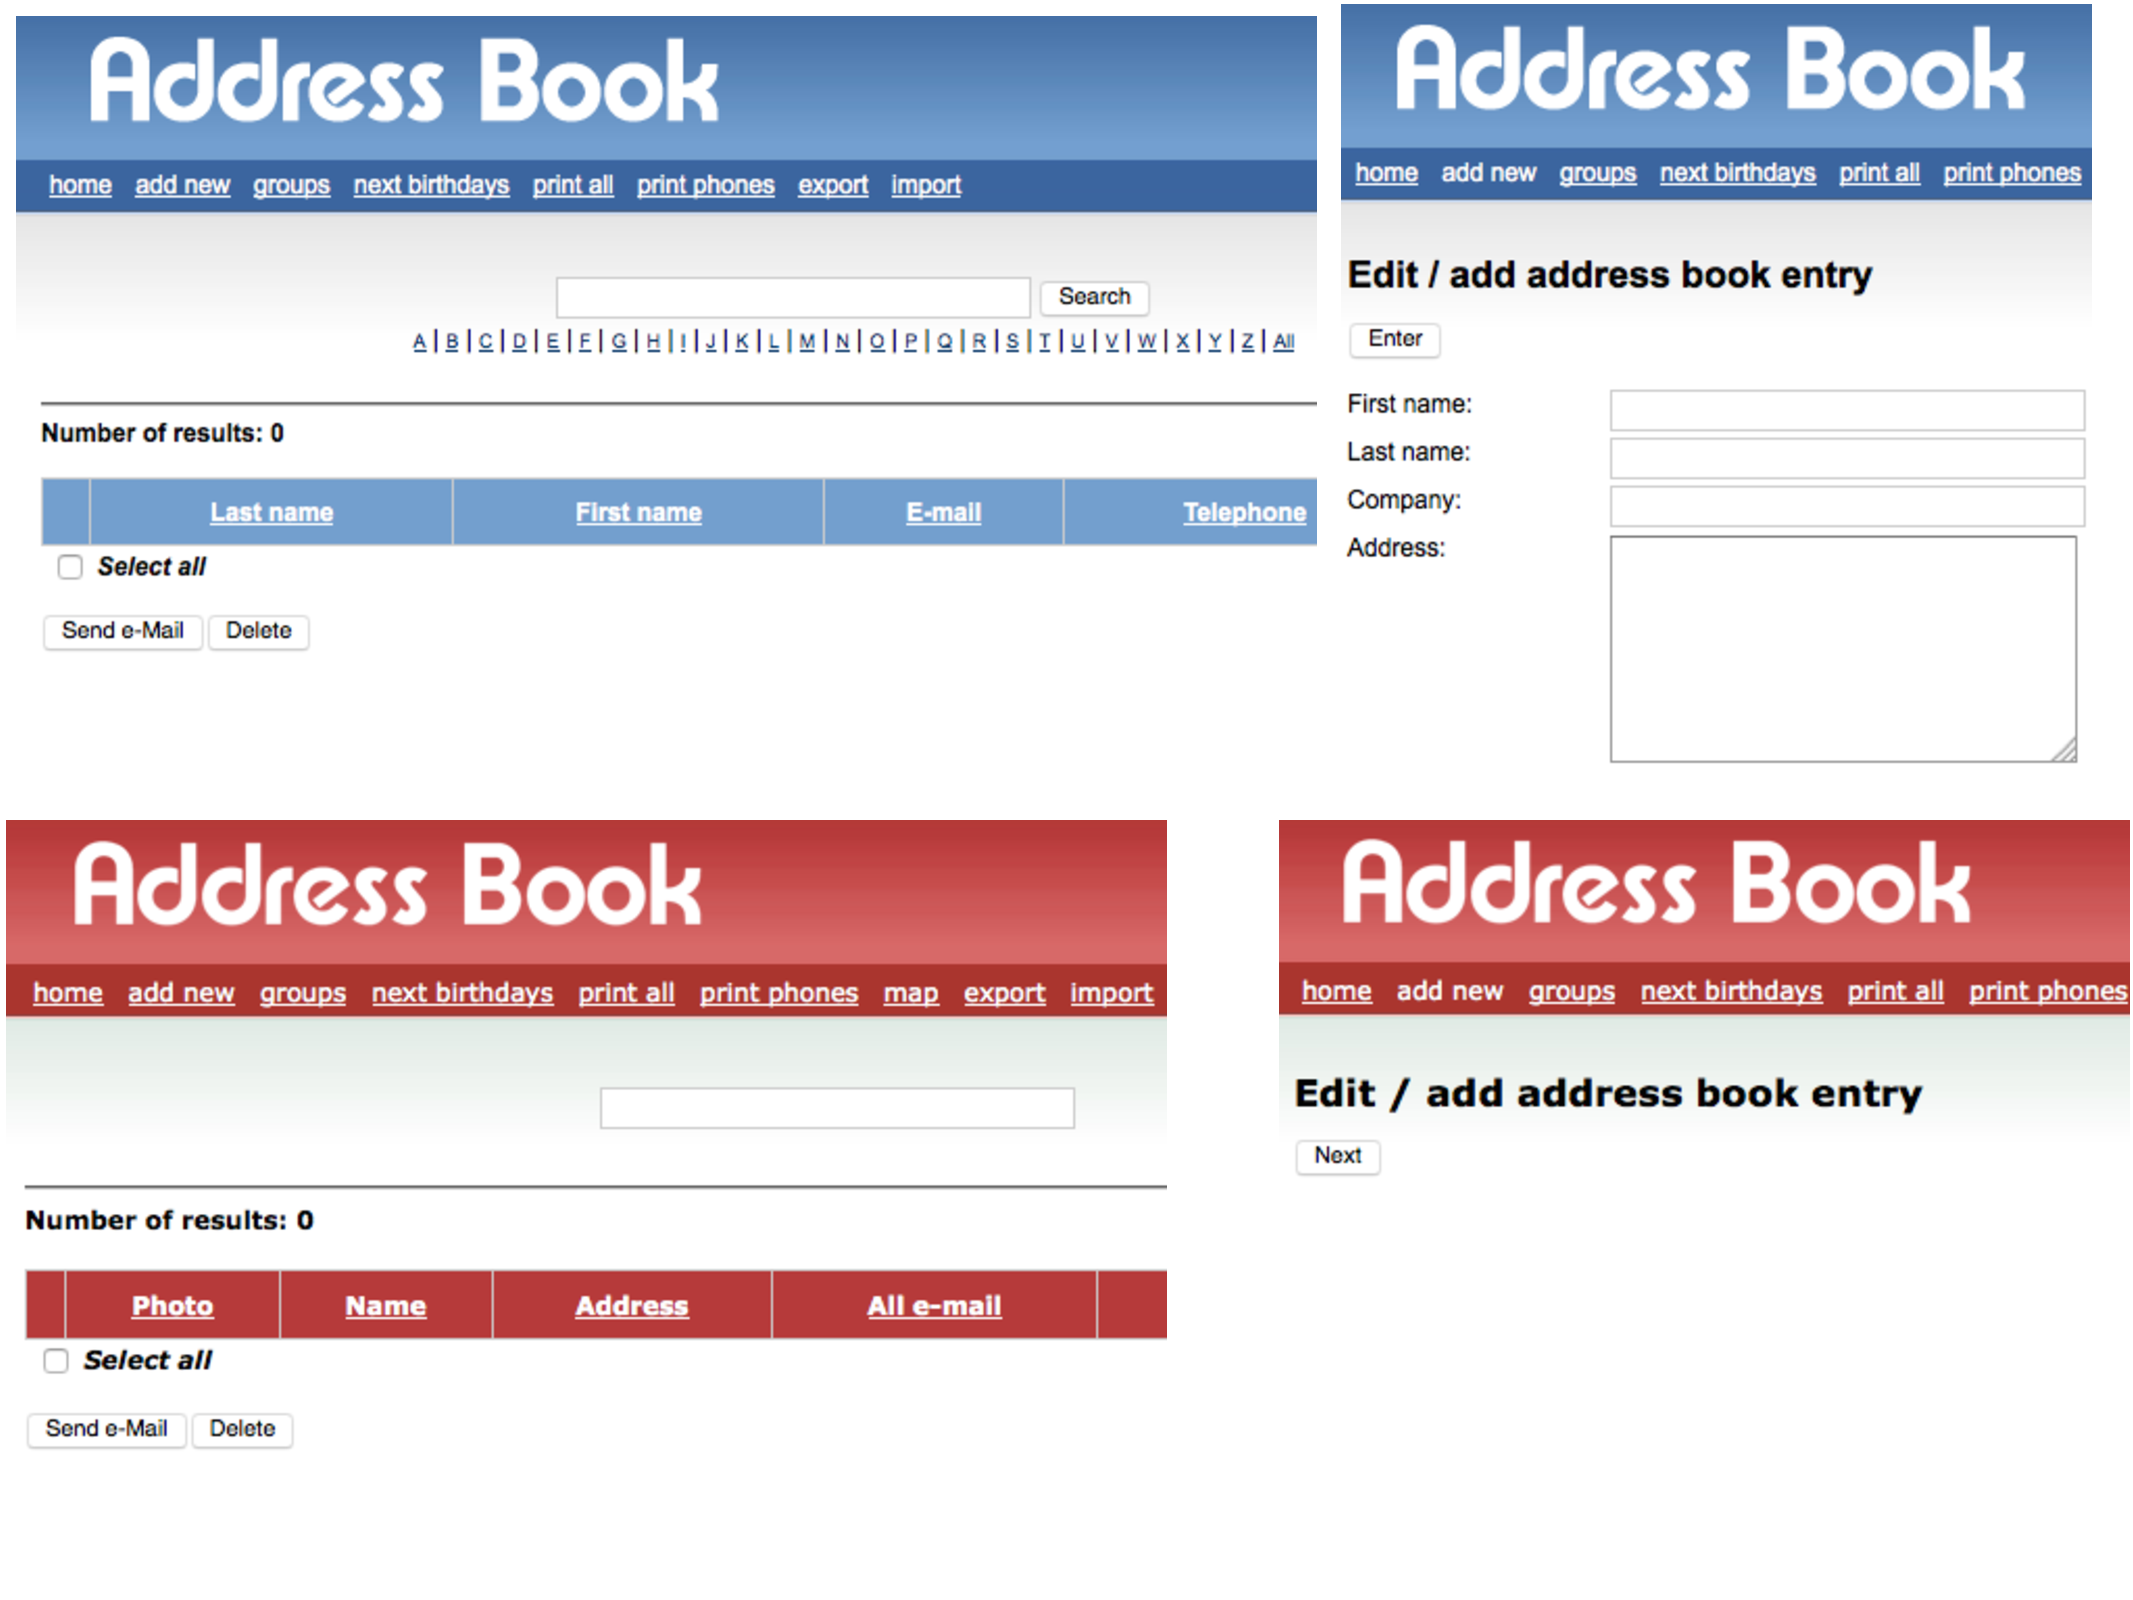
\includegraphics[trim={0cm 2cm 0cm 0cm},clip,scale=0.2]{images/addressbook}
%%%}
%%\caption{AddressBook}
%%\label{addressbook}
%%\end{figure}
%
%\textit{Scenario 2 --- Mis-Selection or Propagated Breakage}.
%We focus on solving the problem due to propagated breakages  because it is very common in web testing due to locators mis-selection. 
%
%We want to make sure that all the locators select the correct elements, respectively.
%
%Two variants: the mis-selection does not cause a state transition (the app remains in the same state), or it does trigger a state transition and leads to a different state.




